\documentclass[10pt,twocolumn,twoside]{IEEEtran}
\usepackage{amsmath}
\usepackage{amsthm}
\usepackage{amsfonts}
\usepackage{amssymb}
\usepackage{bm}
\usepackage{microtype}
\usepackage[margin=0.8in]{geometry}
\usepackage{mathrsfs}
\usepackage{mathtools}
\usepackage{graphicx}
\usepackage{cite}
\usepackage{epstopdf}
\epstopdfsetup{outdir=./}
\DeclareMathOperator*{\argmin}{arg\,min}
\DeclareMathOperator*{\argmax}{arg\,max}
\newtheorem{definition}{Definition}
\newtheorem{lemma}{Lemma}
\newtheorem{theorem}{Theorem}
\newtheorem{problem}{Problem}
\usepackage{algorithm}
\usepackage{algpseudocode}
\newcommand{\vv}[1]{\mbox{\boldmath $#1$}}
\newcommand{\norm}[1]{\left|\left|#1\right|\right|_2}
\newcommand{\showuc}[1]{\MakeUppercase{#1}}
\newcommand{\manuallabel}[2]{\def\@currentlabel{#2}\label{#1}}
\algrenewcommand\alglinenumber[1]{\scriptsize #1}
\def \ETx {\mathcal{E}}
\def \TRx {\Gamma}	
\makeatletter
\let\OldStatex\Statex
\renewcommand{\Statex}[1][3]{%
  \setlength\@tempdima{\algorithmicindent}%
  \OldStatex\hskip\dimexpr#1\@tempdima\relax}
\makeatother
\algdef{SE}[DOWHILE]{Do}{DoWhile}{\algorithmicdo}[1]{\algorithmicwhile\ #1}
\title{}

\author{
\thanks{}
}

\begin{document}
\maketitle
\thispagestyle{empty}
\pagestyle{empty}
\begin{abstract}
\end{abstract}


\begin{IEEEkeywords}
\end{IEEEkeywords}

\section{Notations}
% !TEX root = main.tex
The Transmitter energy arrival instants are marked by $t_i$'s with energy $E^{T}_i$ while the receiver energy arrivals are marked by $r_i$'s with energy $E^{R}_i$ for $i \in \{0,1..\}$. The receiver spends $P$ amount of power to be \textit{on} and no power when it is \textit{off}. Hence each energy arrival $E^{R}_i$ can be viewed as it adds $T^{R}_i=\dfrac{E^{R}_i}{P}$ amount of time for which the receiver can be \textit{on}. The maximum amount of time for which the receiver (and hence the Transmitter) can be \textit{on} till time '.' is given by function $T^{R}(.)$. It can be easily seen that $T^{R}(t)=\sum_{i=0}^{r_i<t}T^{R}_i$. Similarly the maximum energy harvested at the transmitter till time '$t$' is given by function $E^{T}(t)=\sum_{i=0}^{t_i<t}E^{T}_i$. The rate of bits transmition with power '.', given by function $g(.)$ is assumed to follow the following properties as proposed in \cite{Yang} 
\begin{align}
&P1) g(0)=0\text{ and }\lim_{x\rightarrow \infty} g(x)\rightarrow \infty.
\\
&P2) g(x)\text{ is concave in nature with } x.
\\
&P3) g(x)\text{ is increasing with } x.
\\ 
&P4) g(x)/(x) \text{ is monotonically decreasing with } x.
\end{align}

For convenience of presentation, we also follow the following convention : we use the notation $\stackrel{L1}{=}$ or $\stackrel{(1)}{=}$ or $\stackrel{P1}{=}$ or $\stackrel{T1}{=}$ to indicate that the equality "$=$" follows from Lemma 1 / Equation (1) / Property 1 / Theorem 1 respectively (same for inequalities).

\section{OPTIMAL OFFLINE ALGORITHM FOR ENERGY HARVESTING TRANSMITTER AND ENERGY LIMITED RECEIVER}
% !TEX root = ICC.tex
We consider an off-line scenario, which means we know all $t_i$'s and $\ETx_i$'s, non causally. We assume that the receiver harvests energy only once (say of amount $E$) at time $r_0=0$. Hence, the receiver (and so does the transmitter) can be \textit{on} for a maximum period of $\TRx_0=\frac{E}{P_r}$. We also assume that an infinite battery capacity is available both at the transmitter and the receiver to store the harvested energy. Our objective is to complete transmission (transmit $B_0$ bits) as early as possible. This is stated as an optimization problem below.

%The transmitter is supposed to transmit all $B_0$ bits in as minimum time as possible. The problem is formally stated below.
\begin{problem}
\begin{align}
&\min_{\{\textbf{p},\textbf{s},N\}}			&& T
\\
&\text{subject to} 				&& B(T)=B_0, 
\label{pb1_constraint_bits}
\\
&     										&& U(t)\le \mathcal{E}(t)  		&&& \forall \; t\;\in\;[0,T], \label{pb1_constraint_energy}
\\
&    										&& \displaystyle\sum_{\mathclap{i=1:p_i\neq 0}}^{N}(s_{i+1}-s_i)\le \TRx_0.
\label{pb1_constraint_time}
\end{align}
\end{problem}
Constraint \eqref{pb1_constraint_energy} means that we cannot use more than available energy at any point of time till we finish transmission. \eqref{pb1_constraint_time} implies that the maximum duration of transmission cannot exceed $\TRx_0$. Note that the maximum transmission duration would reduce to $(s_{N+1}-s_1)$, as we shall see in Lemma \ref{lemma_nobreaks}.  

Before describing an algorithm to solve Problem 1, we state the following Lemmas, which shall help us construct our algorithm.
\input{propositionsICC}
\input{Algo1_proofICC}
% !TEX root = OptimalOfflineICC.tex

%Summarising the results of Lemmas \ref{lemma_increasing_power}-\ref{transmission_duration}, the optimal policy $\{\textbf{p},\textbf{s},N\}$ may change transmission powers only at energy arrival epochs i.e. $\forall 1<i<N+1,\ s_i=t_j$ for some $j$. At these epochs, it exhausts the total energy available i.e. $U(s_i)=\ETx(s_i^-)$. The transmission powers are also non-decreasing with time and the optimal policy exhausts the total `receiver time' time allowed, if it does not start transmitting from origin.
%
%Now that we have gained some knowledge regarding the structure of the optimal policy, we consider an example to approach Problem 1. 

We next propose a procedure which gives a feasible solution satisfying most\footnote{The initial feasible solution, satisfies all structures, except the one in Lemma \ref{transmission_duration}.} of the necessary structures of the optimal policy.

\textbf{INIT\_POLICY, Initial Feasible solution}:

\textit{Step1:} Identify the first energy arrival instant $t_n$, so that using $\ETx(t_n)$ energy and $\TRx_0$ time, $B_0$ or more bits can be transmitted with a constant power (say $p_c$). Solve for $\widetilde{\TRx}_0$ below.
\begin{align}
&\TRx_0\left(\dfrac{\ETx(t_n)}{\TRx_0}\right)\ge B_0, \widetilde{\TRx}_0\left(\dfrac{\ETx(t_n)}{\widetilde{\TRx}_0}\right)= B_0, p_c = \dfrac{\ETx({t_n})}{\widetilde{\TRx}_0}.
\label{INIT_POLICY_time}
\end{align}
 
\textit{Step2:} Identify the first time instance, say $T_{start}$, such that transmission with $p_c$ for $\widetilde{\TRx}_0$ time, starting from $T_{start}$ is feasible with energy constraint \eqref{pb1_constraint_energy}. Set $T_{stop} = T_{start} + \widetilde{T}_0$. This transmission policy $p_c$, will encounter atleast one energy arrival epoch (call it $t_q$), where $U(t_q) = \ETx(t_q^-)$ (See Fig. \ref{straight}). If $U(T_{stop}) = \ETx(T_{stop}^-)$ as shown in Fig. \ref{straight}(a), then terminate with $p_c$. Otherwise, set $\widetilde{B} = (T_{stop} - t_q)g(p_c)$, which denotes the number of bits to be sent after time $t_q$. Then apply Algorithm 1 from \cite{Yang} from time $t_q$ with $\widetilde{B}$ bits to transmit (shown in Fig. \ref{straight} (b)). Update $T_{stop}$, where this policy ends. Note that, by property of Algorithm 1 from \cite{Yang}, $U(T_{stop}) = \ETx(T_{stop}^-)$.

Now, we describe the algorithm in steps. In any iteration, let $t_{l}$ and $t_{r}$ be the first and last energy arrival epochs where the power of transmission changes. $p_l$ and $p_r$ are the transmission power before $t_l$ and after $t_r$ respectively. $T_{start}$ and $T_{stop}$ are the start and finish time of policy, found in any iteration. $t_l, t_r, p_l, p_r, T_{start}, T_{stop}$ get updated to $t_l', t_r', p_l', p_r', T'_{start}, T'_{stop}$ over a iteration. 
%The policy found by the Algorithm in-between time $t_l$ and $t_r$ is stored in array \textbf{p} and \textbf{s}. 
The possible cases that can happen in an iteration of the Algorithm are shown in Fig. \ref{figure_Algorithm1}.
\begin{figure}
\centering
  \centerline{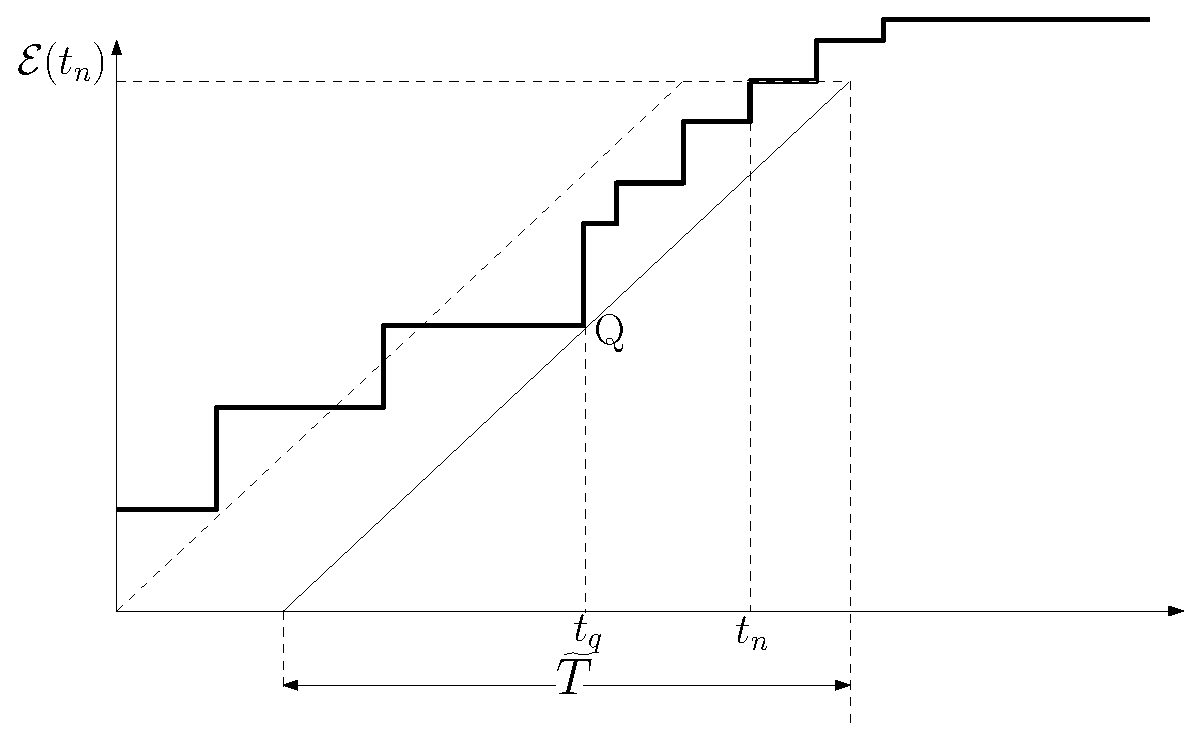
\includegraphics[width=8cm]{straight.eps}}
\caption{Figure showing point $t_q$.}\label{straight}
\end{figure}




\textbf{Algorithm 1}:

\textit{Step3:} Increase $p_r$ till it hits the boundary of energy constraint \eqref{pb1_constraint_energy} as shown in Fig. \ref{figure_Algorithm1}(a). Make this power $p_r'$ and the epoch where it hits \eqref{pb1_constraint_energy} as $t_r'$. So, $U(t_r') = \ETx(t_r'^-)$. Set $T_{stop}'$ to where this policy ends. Calculate $p_l'$ such that decrease in bits transmission from $p_r$ to $p_r'$ is compensated by $p_l'$.
\begin{align}
&\nonumber g(p_r)(T_{stop}-t_r)-g(p_r')(T_{stop}'-t_r')\\
&=g(p_l')\frac{\ETx(t_l'^-)}{p_l'}-g(p_l)(t_l-T_{start}).
\label{eq_example1}
\end{align}

\textit{Step4}: If $p_l'$ is feasible, which is the case shown in Fig. \ref{figure_Algorithm1}(a), set $T_{start}'=t_l-\frac{\ETx(t_l'^-)}{p_l'}$, $t_l'=t_l$. Iterate to \textit{Step3}. 

If $p_l'$ is not feasible, as shown in Fig. \ref{figure_Algorithm1}(b), then $p_l'$ is increased until it becomes feasible. $t_l'$ is set to the first instance where $U(t_l') = \ETx(t_l'^-)$ as shown in Fig. \ref{figure_Algorithm1}(c). Similar to \textit{Step3}, calculate $p_r'$ such that the policy transmits $B_0$ bits and update $p_r',T_{stop}'$ accordingly. Note that $t_r'=t_r$. Iterate to \textit{Step3}.




\textit{Step5:} Going back to \textit{Step3}, suppose $p_r$ could be increased till infinity without violating \eqref{pb1_constraint_energy}. This happens when there in no energy arrival between $t_r$ and $T_{stop}$, as shown in Fig. \ref{figure_Algorithm1}(d). In this case, set $p_r'$ to the transmission power at $t_r^-$, $t_r'$ to epoch where $p_r'$ starts and $T_{stop}'=t_r$. Similar to \textit{Step3}, calculate $p_l'$ and proceed to \textit{Step4}. 

\textit{Termination}: If in any iteration, at the end of \textit{Step4}, $T_{stop}' - T_{start}' \ge \TRx_0$ or $T_{start}' = 0$, then terminate. If $T_{start}' = 0$, then output with the policy found along the Algorithm. If not, calculate $T_{start}'$ and $T_{stop}'$, according to the equations,
\begin{align}
&\nonumber (t_l-T_{start}')\frac{\ETx(t_l^-)}{t_l-T_{start}'}+(T_{stop}'-t_r)\frac{\ETx(T_{stop}^-)}{T_{stop}'-t_r}\\
&=g(p_l)(t_l-T_{start})+g(p_r)(T_{stop}-t_r)\\
&T_{stop}'-T_{start}'=\TRx_0.
\label{eq_termination}
\end{align}
Update $p_l'=\frac{\ETx(t_l^-)}{t_l-T_{start}'}$, $p_r'=\frac{\ETx(T_{stop}^-)}{T_{stop}'-t_r}$, $t_l'=t_l,t_r'=t_r$. Output with this policy. 

Next Lemma shows that point $t_q$ selected by INIT\_POLICY is a 'good' starting solution.
\begin{lemma}
In every optimal solution, at energy arrival epoch $t_q$, $U(t_q)=\ETx(t_q^-)$.
\label{lemma_Q}
\end{lemma}
%Suppose we are given that the receiver can be \textit{on} for a maximum duration of $\TRx_0$. Our goal is to find a transmission policy so that we can minimize the total time at which the transmission of all $B_0$ bits is completed. To do this, we shall first find a feasible solution i.e. one which satisfies all constraints (\ref{pb1_constraint_bits})-(\ref{pb1_constraint_time}) and keep improving upon it, until we have a solution that follows all structural results in Lemma \ref{lemma_increasing_power}-\ref{transmission_duration} (as shown in Theorem \ref{th_algo1_1} later,  these Lemmas form a sufficient condition as well).

%We need an initial feasible solution to begin with. For this, we find the minimum energy required by the transmitter so that the transmission can be completed in duration $\TRx_0$ with a constant power. That is, the first $\ETx(t_n)$ such that
%\begin{equation}
%\TRx_0 g\left(\frac{\ETx(t_n)}{\TRx_0}\right)\geq B_0.
%\end{equation}
%Let $\widetilde{\TRx}_0\le \TRx_0$ be the time duration such that
%\begin{equation}
%\widetilde{\TRx}_0 g\left(\frac{\ETx(t_n)}{\widetilde{\TRx}_0}\right)=B_0.
%\end{equation}
%Let $p_c=\frac{\ETx(t_n)}{\widetilde{\TRx}_0}$. We try to transmit with $p_c$ power starting at time $t=0$. If it does not violate the energy constraint (\ref{pb1_constraint_energy}), we are done with the optimal solution and our transmission is completed in $\widetilde{\TRx}_0<\TRx_0$ time.
%
%If not, we start the transmission at the earliest possible time, such that the transmission with $p_c$ for $\widetilde{\TRx}_0$ time is feasible with respect to (\ref{pb1_constraint_energy}). This transmission policy, will encounter atleast one epoch where total energy consumed till that epoch is equal to the total energy harvested upto it. Let time $t_q$ be the first point where this happens. Let $R$ and $S$ denote the starting and ending time, respectively, of transmission with power $p_c$. Clearly, $S-R=\widetilde{\TRx}_0$. This is shown in Fig. \ref{straight} (a).  Till now we have not argued why we chose such a policy to start with. In fact, Lemma \ref{lemma_Q} shows that this starting solution is a `good' estimate of policy at and before time $t_q$, as both the optimal policy and the above policy run out of all their energy at epoch $t_q$. 
%
%Now, according to Lemma \ref{lemma_energy_consumed}, the optimal policy must finish all available energy when it stops transmission. If transmitting with $p_c$ power does use up all the energy (Fig. \ref{straight} (a)), then we accept the constant power transmission with $p_c$ as our initial policy (line number \ref{init_policy_CP} in Algorithm \ref{init_policy}). If it does not finish up all of $\ETx(t_n)$ with $p_c$ till the end of transmission (shown in Fig. \ref{straight} (b)), we choose a better policy after time $t_q$. Let $\widetilde{B}$ bits be transmitted with power $p_c$ until $S$, which is calculated in line number \ref{init_policy_bits_t_q} of procedure INIT\_POLICY in Algorithm \ref{init_policy}. Now, we require our transmission policy to send $\widetilde{B}$ bits after time $t_q$, in as little time as possible (and of course, before $S$), keeping in mind that the policy should use all $\ETx(t_n)$ amount of energy till it finishes. Algorithm 1 in \cite{Yang} does the job for us. Hence in this case, we choose transmission with $p_c$ till $t_q$ and then the solution of Algorithm 1 in \cite{Yang} after time $t_q$. 
%\begin{algorithm}
%%\algsetup{linenosize=\tiny}
%%\alglinenumber{linenosize=\scriptsize}
%\caption{Procedure to find initial feasible policy to Problem 1 for Algorithm 2}
%
%\footnotesize%\scriptsize
%\label{init_policy}
%\begin{algorithmic}[1]
%\State \textbf{Initialization}: $B_0$, $\TRx_0$
%\Procedure{INIT\_POLICY}{}
%
%\State $n=\displaystyle \argmin_k\left(\left\{t_k | \TRx_0 g\left(\frac{\ETx(t_k)}{\TRx_0}\right)\geq B_0\right\}\right)$ \label{init_policy_Etn}
%
%\State Solve for $\widetilde{T}: \widetilde{T}g\left(\dfrac{\ETx(t_n)}{\widetilde{T}}\right) = B_0$\label{init_policy_CP_time}
%
%\State $p_c=\dfrac{\ETx(n)}{\widetilde{T}}$
%
%\State $q=\displaystyle \argmin_k\ ( \{ t_k | ((\ETx(t_k) - p_ct_k) + p_ct_j) \leq \ETx(t_j),$
%
%$			 						\qquad \qquad \qquad \forall j\in[0,n]  \} )$
%\label{init_policy_t_q}
%\State $R=t_q-\dfrac{\ETx(t_q)}{p_c}$, $S=t_q+\dfrac{\ETx(t_n)-\ETx(t_q)}{p_c}$
%
%\If {$\ETx(t_n)<\ETx(S^-)$}
%	\State $\widetilde{B}=g(p_c)(S-t_q)$\label{init_policy_bits_t_q}  
%	\State $\{\textbf{p},\textbf{s},N\}\gets$  Apply Algorithm 1 in \cite{Yang} to 	minimize time of
%		\Statex   transmission of $\widetilde{B}$ bits  after time $t_q$ assuming	a  total of $\ETx_{q}$   
%		\Statex amount of energy available at $t_q$. 
%	\State\Return $\{\{p_c,\textbf{p}\},R,\textbf{s}\},N+1\}$ \label{init_policy_Yang}
%	 	\Statex (Transmission with $p_c$ from $R$ to $t_q$ and then with
%	 	\Statex policy $\{\textbf{p},\textbf{s},N\}$)
%\Else 
%	\State\Return $\{\{p_c,p_c\},\{R,t_q,S\},2\}$ \label{init_policy_CP}
%\EndIf
%\EndProcedure
%\end{algorithmic}
%\end{algorithm}


%\begin{proof}
%We shall prove this by contradiction. First, we make the following claims:
%
%\textbf{Claim 1:} Every optimal transmission policy begins transmission at or before time $R$.
%
%Since, $S-R=\widetilde{\TRx}_0\le \TRx_0$, by Lemma \ref{transmission_duration}, if a transmission policy has to finish before $S$, it has to start before time $\max(S-\TRx_0,0) \le \max(R,0)=R$. 
%
%%Since we are transmitting all the bits at the maximum possible power, no policy that starts after $R$ can finish before $S$. Therefore, any policy that starts after $R$ cannot be optimal.
%
%\textbf{Claim 2:} Every optimal transmission policy ends transmission at or before time $S$.
%%This follows immediately from the fact that the policy is optimal.
%
%If it does not, then constant power policy $p_c$ finishing at $S$ will contradict its optimality.
%%Let $t_q$ equal to time $t_i$ for some $i\in\mathbb{N}$. 
%
%Suppose we have an optimal transmission policy, say $X$,$\{\bm{p},\bm{s},N\}$, that does not exhaust all its energy at time $t_q$ i.e. $U(t_q)<\ETx(t_q^-)$. Then, by Lemma \ref{lemma_energy_consumed}, it does not change its transmission power at $t_q$. Let the transmission power of $X$ be $p_{j-1}$ at $t_q$ and $p_{j-1}$ starts from $s_{j-1}$ and goes till $s_j$. Now, $s_j<S$ by \textit{Claim 2}. Further, power $p_c$ exhausts all energy by $t_q$. So,
%\begin{align}
%&p_c(t_q-R)=\ETx(t_q^-)\label{eqlemmaQ1}.
%\end{align}
%But, by constraint (\ref{pb1_constraint_energy}),
%\begin{align}
%&p_c(t_q-R)+p_c(s_j-t_q)\le \ETx(s_j^-),
%\\
%& p_c(s_j-t_q)\stackrel{(\ref{eqlemmaQ1})}{\le} \ETx(s_j^-)-\ETx(t_q^-),
%\\
%& p_c(s_j-t_q)< \ETx(s_j^-)-U(t_q)=p_{j-1}(s_j-t_q),
%\\
%& p_c<p_{j-1} .\label{eqlemmaQ2}
%\end{align}
%If ${j-1}= 1$, then power at $t_q$ is the first transmission power $p_1$. But then by \eqref{eqlemmaQ2}, $p_1 > p_c$. By the definition of $p_c$, we must have $s_{1} > R$, but this will contradict \textit{Claim 1}.
%
%So ${j-1}\ge 2$, which means that the power of transmission must change at least once between $R$ and $t_q$. By Lemma \ref{lemma_energy_consumed}, $X$ has used all energy by $s_{j-1}$ and $s_{j}$ as well. So, $p_{j}(\ETx(s_{j}^-)-\ETx(s_{j-1}^-))$ is the maximum energy available between time $s_{j-1}$ and $s_{j}$. If $R<s_{j-1}$, then $p_c$ (by \eqref{eqlemmaQ2}) uses more energy, than available between $s_{j-1}$ and $s_{j}$, which is not possible. If $s_{j-1}\le R$ then $p_{j-1}$ uses more than maximum energy available (given by $p_c(t_q-R)=\ETx(t_q^-)$ ) between time $R$ and $t_q$, violating energy constraint \eqref{pb1_constraint_energy}. 
%
%Therefore, every optimal transmission policy must use all energy till epoch $t_q$. 
%
%%If the optimal policy does have a power higher than $p_c$ at $t_q$, then it must have the same power of transmission either from some epoch, say $t_k$, or from the beginning of transmission. If $t_k>R$, we can show that $p_c$ becomes infeasible with respect to energy constraint (\ref{pb1_constraint_energy}) at $t_k$. If $t_k<R$, $p$ becomes infeasible with energy constraint \eqref{pb1_constraint_energy} at time $R$. Now, only thing left is the optimal policy begins transmission with power $p$. If so, then it has to begin transmission after time $R$ which follows from equation (\ref{eqlemmaQ2}). This violates \textit{Claim 1}. Therefore every optimal transmission policy must use all energy till epoch $t_q$.
%\end{proof}

%Now that we have an initial feasible solution, we shall proceed to improve upon this policy as follows. The formal algorithm is presented as Algorithm \ref{Algorithm1}. We explain the procedure by an example. Assume that the starting feasible solution is given by the constant power policy, as shown by dotted line in Fig. \ref{figure_example_Algorithm1} (a), where $t_q=t_2$. We first assign the following initial values for the initial feasible policy - transmission power left of $t_2$ as $p_l=p_c$, power right of $t_2$ as $p_r=p_c$, start time $T_{start}=R$, stop time $T_{stop}=S$, epoch at which $p_l$ ends as $t_l=t_2$, epoch at which $p_r$ starts as $t_r=t_2$. Now, we increase $p_r$, keeping $t_r$ fixed, till it reaches $p_r'$ which hits epoch $t_3$, as shown by the solid line in Fig \ref{figure_example_Algorithm1} (a). As in total we need to transmit $B_0$ bits, the decrease in bits transferred by $p_r$ to $p_r'$ (RHS of \eqref{eq_example1}) is compensated by calculating appropriate $p_l'$ according to the following equation, where LHS represents the increase in bits transmitted from $p_l$ to $p_l'$.
%\begin{align}
%&g(p_l')\frac{\ETx(t_l^-)}{p_l'}-g(p_l)(t_l-T_{start})=-g(p_r)(T_{stop}-t_r)\nonumber\\
%&+g(p_r')(\mathcal{P}(t_r,t_3))\frac{\ETx(T_{stop}^-)-ETx(t_r^-)}{\mathcal{P}(t_r,t_3)}.
%\label{eq_example1}
%\end{align}   
%Having got a feasible $p_l'$, as shown in Fig. \ref{figure_example_Algorithm1} (a), we assign $T_{start}'$ with the point where $p_l'$ starts, $T_{stop}'$ with the point where $p_r'$ ends. $t_r'$ gets the value $t_3$ and $t_l'$ remains same as $t_l=t_2$. Note that parameters $\{T_{start}',T_{stop}',t_l',t_r',p_l',p_r'\}$ define the policy at the end of first iteration. 
%
%In the next iteration, the portion of transmission between $t_l'=t_2$ to $t_r'=t_3$ is not updated. In this iteration, we try to increase $p_r'$ about $t_r'$ till it hits the feasibility equation \eqref{pb1_constraint_energy} of energy. $p_r'$ could virtually be increased to infinity. But transmission with infinite power for 0 time does not transmit any bits. So we assign $t_r''=t_2$ and $p_r''=\mathcal{P}(t_2,t_3)$. With this change in $p_r'$ to $p_r''$, we again calculate $p_l''$ which compensates the decrease in bits transferred after $t_r'$. But the calculated $p_l''$ becomes infeasible at $t_1$ as shown in Fig. \ref{figure_example_Algorithm1} (b). Hence, we set $p_l''$ to the maximum feasible power $\mathcal{P}(t_1,t_2)$ as shown in Fig. \ref{figure_example_Algorithm1} (c). With this $p_l''$, we re-calculate $p_r''$, so as to transmit $B_0$ bits in total. $t_l''$ is assigned to $t_1$, $t_r''$ remains $t_3$. $T_{start}''$ and $T_{stop}''$ as calculated to values marked in Fig. \ref{figure_example_Algorithm1} (c). The final policy at the end of second iteration is shown by solid line in Fig. \ref{figure_example_Algorithm1} (c). Like this, we continue to the third iteration, by improving the policy (to finish earlier) before $t_l''$ and after $t_r''$ and so on.
%
%
%\begin{figure}
%\centering
%  \centerline{\includegraphics[width=8cm]{example_algo1.eps}}
%\caption{Figures showing (a) first  and (c) second iteration of the Algorithm \ref{Algorithm1} through an example. (b) representes an intermidiate step in second iteration. In any diagram, the dashed line represent previous iteration policy and solid line is the present iteration policy.}\label{figure_example_Algorithm1}
%\end{figure}
%
%
%Now we describe the algorithm in steps. In any iteration, let $t_{l}$ and $t_{r}$ be the first and last energy arrival epochs where the power of transmission changes. $p_l$ and $p_r$ are the transmission power before $t_l$ and after $t_r$ respectively. $T_{start}$ and $T_{stop}$ are the start and finish time of the policy, found in any iteration. The policy found by the Algorithm in-between time $t_l$ and $t_r$ is stored in array \textbf{p} and \textbf{s}. The possible cases that can happen in an iteration of the Algorithm are shown in Fig. \ref{figure_Algorithm1}. 
%
%Step1: The Algorithm tries to increase $p_r$ as much as possible till it hits the boundary of energy constraint \eqref{pb1_constraint_energy} as shown in Fig. \ref{figure_Algorithm1}(a). Then the Algorithm calculates the possible power $p_l'$ such that it transmits same number of bits in total with the previous iteration policy, i.e. $B_0$, as shown in line number \ref{algo_bits_left_1} and \ref{algo_bits_left_2} of Algorithm \ref{Algorithm1}. 
%
%Step2: If $p_l'$ is feasible, which is the case shown in Fig. \ref{figure_Algorithm1}(a), the policy changes $p_l$ to $p_l'$ and $p_r$ to $p_r'$ (with $t_r$ to $t_r'$). $T_{start}$ and $T_{stop}$ are changed accordingly to start and end points of $p_l'$  and $p_r'$. 
%
%Step3: If $p_l'$ is not feasible, as shown in Fig. \ref{figure_Algorithm1}(b), then $p_l'$ is set to be the maximum possible feasible power from $t_l$, as shown in Fig. \ref{figure_Algorithm1}(c). Now, $p_r'$ is calculated so as to settle the transmission of equal number of bits as the previous iteration. 
%%We can be sure that $p_r'$ calculated now, would not be infeasible. 
%In this case $t_l$ gets updated to $t_l'$.  
%
%Going back to the first step of the algorithm where we were increasing $p_r$, it could happen, as shown in Fig. \ref{figure_Algorithm1}(d), that $p_r$ can increase to infinity without violating the energy constraint \eqref{pb1_constraint_energy}. This happens when there is no energy epoch between $t_r$ and $T_{stop}$. In this scenario, transmission is stopped at $t_r$,i.e. $T_{stop}$ gets updated to $t_r$ and both $t_r$ and $p_r$ are set to the last values in array \textbf{s},\textbf{p} receptively. This is shown in Fig. \ref{figure_Algorithm1}(d). Now, the Algorithm proceeds to calculate $p_l'$ as done in Step1, and continues as before to check whether $p_l'$ is feasible and decides according to Step2 or Step3.

\begin{figure}
\centering
  \centerline{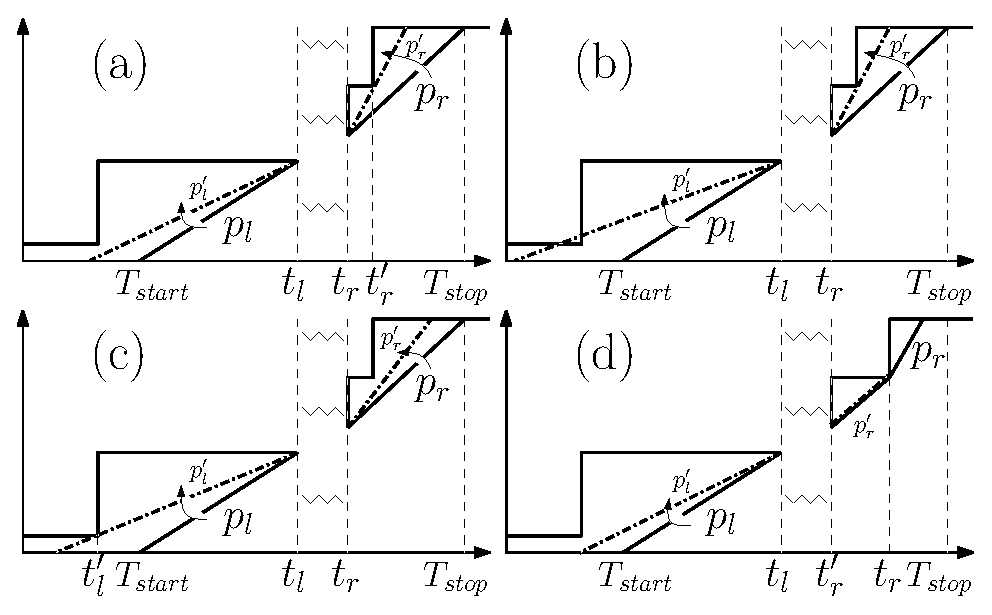
\includegraphics[width=8cm]{Algorithm1.eps}}
\caption{Figures showing any iteration of the Algorithm \ref{Algorithm1}. The solid line represents the transmission policy in the previous iteration. The dash dotted lines in (a), (b), (c), (d) represent the possible configurations of policy in the current iteration.}\label{figure_Algorithm1}
\end{figure}
 
\begin{theorem}
A transmission policy $\{\textbf{p},\textbf{s},N\}$ is an optimal solution to Problem 1 if and only if it satisfies the following structure.
\label{th_algo1_1}
\begin{align}
&\sum_{i=1}^{i=N}g(p_i)(s_{i+1}-s_i)=B_0; 								
\label{claim1}
\\
&p_1\le p_2 ..\le p_N;
\label{claim3}  
\\
&\nonumber s_i=t_j \text{ for some } j, i\in \{2,..,N\} \ \text{ and }
\\
& U(s_i)=\ETx(s_i^-), \forall i\in \{2,..,N+1\};
\label{claim4}
\\
&\nonumber s_{N+1}-s_1=\TRx_0, 	 \ \ \ \ 						\text{ if } s_1>0 \text{ or }
\\
& s_{N+1}\le \TRx_0,				\ \ \ \ \ \ \ \ \ \				\text{ if } s_1=0;
\label{claim2}
\\
&\exists s_j:s_j\in \textbf{s} \text{ and } s_j=t_q.
\label{claim5}
\end{align}
%& \nonumber s_{n+1}=\argmin_{t_i: s_n < t_i \le s_{N+1}} \mathcal{P}(s_n,t_i)=\dfrac{\ETx(t_i^-)-U(s_n)}{t_i-s_n} \	\text{ and }
%\\
%&p_n=\mathcal{P}(s_{n},s_{n+1});\label{claim3}							
%\\
\end{theorem}

\begin{theorem}
The proposed transmission policy is an optimal solution to Problem 1.
\label{th_algo1_2}
\end{theorem}
\begin{proof}
To prove that the policy (say $\{\textbf{p},\textbf{s},N\}$) given by Algorithm \ref{Algorithm1} is optimal, it is sufficient to show that it abides by the structure presented in Theorem \ref{th_algo1_1}.

To begin with, we prove that the power allocations in Algorithm \ref{Algorithm1} are non-decreasing. We prove this by induction. The base case constitutes of showing that, the initial feasible solution has non-decreasing powers. If INIT\_POLICY returns the constant power policy $p_c$ from time $T_{start}$ to $T_{stop}$, then our claim holds. 

Suppose INIT\_POLICY does not return the constant power policy, but applies Algorithm 1 from \cite{Yang} with $\widetilde{B}=B_0-g(p_c)(t_q-T_{start})$ bits to transmit after time $t_q$, then by the properties satisfied by optimal policy presented in \cite{Yang}, we know that the transmission powers would be non-decreasing after time $t_q$. Also, since it is optimal and power $p_c$ transmits $\widetilde{B}$ bits by time $(T_{start}+\widetilde{\TRx}_0)$,  $T_{stop}\le (T_{start}+\widetilde{\TRx}_0)$. Now, we need to prove that transmission power $p_c$ between time $T_{start}$ and $t_q$ is less than or equal to the transmission power just after time $t_q$ (say $p_i$). We prove it by contradiction. Assume that $p_i<p_c$.

Let transmission with $p_i$ end at an epoch $t_i$. $U(t_i)=\ETx(t_i^-)$ by properties of optimal policy in \cite{Yang}. So, energy consumed by $p_c$ between time $t_q$ to $t_i$ is, 
\begin{align}
&p_c(t_i-t_q)>p_i(t_i-t_q)=(\ETx(t_i^-)-\ETx(t_q^-)).\label{eq_1_algo1_modified}
\end{align}
Since, constant power policy with $p_c$ uses all the available energy by $t_q$, the maximum amount of energy available for transmission between $t_q$ and $t_i$ is $\left(\ETx(t_i^-)-\ETx(t_q^-)\right)$. By \eqref{eq_1_algo1_modified}, $p_c$ uses more than this energy and therefore, it is infeasible between time $t_q$ and $t_i$. But, transmission with power $p_c$ is atleast feasible till time $(T_{start}+\widetilde{\TRx}_0)\ge t_i$. So, we reach a contradiction.        
%
%\textit{Case2:} If $t_i>T_{start}+\TRx_0$, then $\ETx(t_i^-)>\ETx(T_{start}+\TRx_0)=\ETx(t_n)$. So, 
%\begin{align}
%g(p_i)(t_i-t_q)&=g\left(\frac{\ETx(t_i^-)-\ETx(t_q^-)}{t_i-t_q}\right)(t_i-t_q)
%\\
%&>g\left(\frac{\ETx(t_n)-\ETx(t_q^-)}{t_i-t_q}\right)(t_i-t_q)
%\\
%&\stackrel{(a)}{>}g\left(\frac{\ETx(t_n)-\ETx(t_q^-)}{T_{start}+\TRx_0-t_q}\right)(T_{start}+\TRx_0-t_q)\label{eq_2_algo1_modified}
%\\
%&=g(p_c)(T_{start}+\TRx_0-t_q)=\widetilde{B}.
%\end{align}
%where %\eqref{eq_2_algo1_modified} 
%$(a)$ follows from \eqref{property_decreasing}. So transmission with $p_i$ from $t_q$ to $t_i$ sends more than $\widetilde{B}$ bits. This is inconsistent with the assumption that the solution we get from Algorithm 1 in \cite{Yang} exactly transmits $\widetilde{B}$ bits after $t_q$. 

Now that we have proved the base case, we assume that transmission powers from Algorithm \ref{Algorithm1} are non-decreasing till its $n^{th}$ iteration. The transmission powers between $t_l$ and $t_r$ do not change from the $n^{th}$ to the $(n+1)^{th}$ iteration, as illustrated in Fig. \ref{figure_Algorithm1}. So, we only need to prove that the transmission power before time $t_l$ is less than the transmission power after $t_l$ and the same for time $t_r$. In the $(n+1)^{th}$ iteration, by the definition of the algorithm either $t_l$ updates or $t_{r}$ updates. Assume $t_l$ gets updated to $t_{l}'$, $p_l$ to $p_l'$, $p_r$ to $p_r'$ and $t_r$ remains same. The proof for $t_r$ getting updated can be done with similar arguments and hence we only show proof of this case. If we show that $p_l<p_l'$ and $p_r>p_r'$, then we are done by induction hypothesis.

If $t_l$ updates and $t_r$ remains same, then we are certain that $p_{r}'>p_r$ by algorithm definition. Now, from $n^{th}$ step to $(n+1)^{th}$ step, the number of bits transmitted after $t_r$ should decrease as $p_{r}'>p_r$ and both $p_r,p_r'$ use same amount of energy by the time they end. So, the number of bits transmitted before $t_l$ must be increasing from $n^{th}$ to $(n+1)^{th}$ iteration. This implies that $p_l'$ must also be less than $p_l$.

In the case where $p_r$ is increased till infinity, and $t_r$ and $p_r$ are updated to their previous values, the powers must remain increasing, since $p'_l <p_l$ and the remaining powers are increasing, by the induction hypothesis. Hence we have proved that the transmission powers are always non-deceasing in the policy being output by Algorithm \ref{Algorithm1}. So it follows structure \eqref{claim3}, \eqref{claim4}.

%Now, we show that transmission powers follow structure \eqref{claim3}. Assume it does not. Specifically, say $p_1$ does not follow structure \eqref{claim3}. The proof for $p_2,p_3..$ can be done likewise. So, $p_1$ has to be more than the minimum possible power i.e. $p_1>\mathcal{P}(s_1,\tilde{s})$, where $\tilde{s}=\displaystyle\argmin_{t_i: s_n < t_i \le s_{N+1}} \mathcal{P}(t_i,s_n)$. Then the amount of energy used by $p_1,p_2,..$ till epoch $\tilde{s}$ can be lower bounded by $p_1(\tilde{s}-s_1)$, as $p_1>p_2..$ . But the maximum power available till time $\tilde{s}$ is $\ETx(\tilde{s})=\mathcal{P}(s_1,\tilde{s})(\tilde{s}-s_1)>p_1(\tilde{s}-s_1)$, which is more than what is spent by $p_1$. Hence we reach a contradiction and therefore $p_1=\mathcal{P}(s_1,\tilde{s})$.

Next, we show that Algorithm \ref{Algorithm1} always terminates to a policy i.e it cannot continue indefinitely. If the policy output by INIT\_POLICY, is the constant power policy $p_c$, then initially $(T_{stop}-T_{start})=\widetilde{\TRx}_0$, where $\widetilde{\TRx}_0$ is defined in \eqref{INIT_POLICY_time}. Also, $\widetilde{\TRx}_0\le \TRx_0$ by monotonicity of $g(p)/p$ in \eqref{property_decreasing}.

Suppose Algorithm \ref{init_policy} returns policy with power $p_c$ till $t_q$ and then policy from Algorithm 1 in  \cite{Yang}, then $T_{stop}\le (T_{start}+ \TRx_0)$. 

From the arguments presented while proving non-decreasing powers of Algorithm \ref{Algorithm1}, we can also conclude that $T_{start}$ and $T_{stop}$ always decrease across the iterations. Further, in all the cases of Algorithm \ref{Algorithm1}, described in Fig. \ref{figure_Algorithm1} (a) (b) (d), we can show, using Lemma \ref{lemma_increase_time}, that $(T_{stop}-T_{start})$ always increases across the iterations in finite steps. As, in initial iteration $(T_{stop}-T_{start})\le \TRx_0$ and $T_{start}\ge 0$, after some finite number of iterations, $(T_{stop}-T_{start})$ will increase beyond $\TRx_0$, or $T_{start}$ would reach 0 and Algorithm \ref{Algorithm1} would terminate.

We argue the satisfaction of structure \eqref{claim2} next. Let $\{T_{start}',T_{stop}',p_l',p_r',t_l',t_r'\}$ be the parameters of Algorithm in the termination iteration and $\{T_{start},T_{stop},p_l,p_r,t_l,t_r\}$ be the values in the previous iteration. For the case where algorithm terminates with $T_{start}'=0$ and $T_{start}'-T_{stop}'\le\TRx_0$, the policy being output satisfies \eqref{claim2}. 

Suppose, the algorithm terminates with $T_{stop}-T_{start}>\TRx_0$. The possible valid configurations can be one of the three shown in Fig. \ref{figure_Algorithm1} (a), (c), (d). Note that $\ETx(T_{stop}^-)=\ETx(T_{stop}'^-)$ in all the cases. (In case Fig. \ref{figure_Algorithm1} (d) we can assume that $T_{stop}'=t_r^+$ and transmission exists after $t_r$, but with infinite power. Since transmitting with infinite power for $0$ time does not transmit any bits, we would transmit the same number of bits, as we did prior to this modification). Thus, the termination policy and the one in previous iteration satisfy the conditions of Lemma \ref{lemma_increase_time}. So, $(T_{stop}'-T_{start}')>(T_{stop}-T_{start})$. Since $(T_{stop}'-T_{start}')>\TRx_0>(T_{stop}-T_{start})$, there must exist a solution to \eqref{eq_termination}. Let the policy obtained from the solution start and end at $T_{start}''$ and $T_{stop}''$. Then $T_{stop}''$ and $T_{start}''$ would lie in-between $T_{stop}$,$T_{stop}'$ and $T_{start}$,$T_{start}'$ respectively. Also, $T_{stop}''-T_{start}''=\TRx_0$. So, structure \eqref{claim2} is satisfied.

Now, according to the definition of $t_n$ and $t_q$ in INIT\_POLICY, $t_q\le t_n$ and $\ETx(t_q^-)<\ETx(t_n)$. Since $t_n$ is defined as the first energy arrival epoch with which $B_0$ bits can be transmitted in $\TRx_0$ time, any transmission policy which ends at or before $t_n$ should take more than $\TRx_0$ time to transmit all of $B_0$ bits. As $t_q\le t_n$, we are guaranteed that no transmission policy can finish at or before $t_q$. Hence in the iterations of the Algorithm \ref{Algorithm1}, $t_r$ can never decrease beyond $t_q$. As $t_q$ is present in the initial solution, $t_q$ always exists in the final solution to Algorithm \ref{Algorithm1}. This verifies structure \eqref{claim5}.  
 
To conclude, all structural results \eqref{claim1}-\eqref{claim5} are satisfied by the policy output by Algorithm \ref{Algorithm1}. Therefore,  by Theorem \ref{th_algo1_1}, Algorithm \ref{Algorithm1} results in an optimal solution.
\end{proof}




\section{ONLINE ALGORITHM FOR ENERGY HARVESTING TRANSMITTER AND RECEIVER}
% !TEX root = ICC.tex
In an online scenario, transmitter and receiver are assumed to have only causal information about energy arrivals i.e. they have no knowledge of future energy harvests. To model a general energy harvesting system, they are further assumed to not have any information about the distribution of future energy arrivals. We propose an algorithm to schedule the transmission of bits in this model. Motivated by \cite{VazeCompetitive}, we use competitive ratio analysis to compare the performance of online policy vs. the optimal offline policy. In this context, we say that our algorithm is $r$-competitive if for all possible energy arrivals at the transmitter $\ETx(t)$ and all possible `time' arrival $\TRx(t)$ at the receiver, the ratio of time taken by the online algorithm (say $T_{\mbox{\scriptsize{online}}}$) to the optimal offline one (say $T_{\mbox{\scriptsize{off}}}$) is bounded by $r$.
\begin{align}
&\displaystyle\max_{\ETx(t),\TRx(t)\hspace{0.5mm} \forall t}\dfrac{T_{\mbox{\scriptsize{online}}}}{T_{\mbox{\scriptsize{off}}}}\le r.
\end{align}
 
\textit{Notation:} The starting time of transmission is denoted by $T_{\mbox{\scriptsize{start}}}$ and the present time is denoted by $t$. The number of bits and energy remaining to transmit at any transmitter energy epoch is represented by $B_{\mbox{\scriptsize{rem}}}$ and $E_{\mbox{\scriptsize{rem}}}$ receptively. We use the same notation $\{\bm{p},\bm{s},N\}$ to denote an onilne policy as described for offline policies.

%The online algorithm that we propose is presented in Algorithm \ref{algo_online}. 
\textit{Online Algorithm:} The Algorithm waits till time $T_{\mbox{\scriptsize{start}}}$ which marks the first energy arrival at transmitter or `time' addition at receiver such that using the energy $\ETx(T_{\mbox{\scriptsize{start}}})$ and time $\TRx(T_{\mbox{\scriptsize{start}}})$, $B_0$ or more bits can be transmitted.
\begin{equation}
T_{\mbox{\scriptsize{start}}}=\min\ t \ s.t.\  \TRx(t)g\Bigg{(} \dfrac{\ETx(t)}{\TRx(t)}\Bigg{)}\ge B_0.\label{online_T_start}
\end{equation}

To begin with, the transmitter equally divides $\ETx(T_{\mbox{\scriptsize{start}}})$ energy among all $B_0$ bits i.e. the first transmission power $p_1$ is set such that,
\begin{align}
&\frac{\ETx(T_{\mbox{\scriptsize{start}}})}{p_1}g(p_1)=B_0.
\label{eq_online_first_power}
\end{align}

By definition of $T_{\mbox{\scriptsize{start}}}$ in \eqref{online_T_start}, we know that transmission with power $p_1$ is going to finish in less than or equal to  $\TRx(T_{\mbox{\scriptsize{start}}})$ time.

If and when energy is harvested at the transmitter, the transmission power is changed. The total unused energy left at such an instant, $E_{\mbox{\scriptsize{rem}}}$, is equally divided among the bits left to transmit i.e. $B_{\mbox{\scriptsize{rem}}}$i.e. 
\begin{equation}
\frac{E_{\mbox{\scriptsize{rem}}}}{p} g(p)= B_{\mbox{\scriptsize{rem}}}.\end{equation}
Note that we do not change our transmission power when there is a `time' arrival at the receiver after $T_{\mbox{\scriptsize{start}}}$, because there is sufficient receiver time already available to finish transmission. Also, the online algorithm changes its transmission power at every transmitter energy epoch after $T_{\mbox{\scriptsize{start}}}$ unlike the optimal offline policy. 

\textit{Example:} Fig. \ref{figure_online_example} shows output of online algorithm, for certain $\ETx(t)$ and $\TRx(t)$. Initially, suppose $B_0$ bits are not possible to be sent with $\ETx_0$ energy  within $\TRx_0$ time i.e. $\TRx(t_0)g\left( \dfrac{\ETx(t_0)}{\TRx(t_0)}\right)<B_0$. Further, $\TRx(r_1)g\left( \dfrac{\ETx(r_1)}{\TRx(r_1)}\right)<B_0$ and $\TRx(t_1)g\left( \dfrac{\ETx(t_1)}{\TRx(t_1)}\right)<B_0$. But, $\TRx(r_2)g\left( \dfrac{\ETx(r_2)}{\TRx(r_2)}\right)>B_0$. So, transmitter starts its transmission at $T_{\mbox{\scriptsize{start}}}=r_2$ with a power $p_1$ such that at rate $g(p_1)$, $B_0$ bits can be sent in $\ETx(r_2)/p_1$ time, as given in \eqref{eq_online_first_power}. At time $t=r_2$, transmitter expects transmission to finish by $r_2+\ETx(r_2)/p_1$ time. But, due to new energy arrival at time $t_2$, it can finish transmission earlier at a higher rate than $p_1$. At $t=t_2$, energy stored at transmitter is $E_{\mbox{\scriptsize{rem}}}=\ETx(r_2)+\ETx_2-(t_2-r_2)p_1$ and bits left to transmit is $B_{\mbox{\scriptsize{rem}}}=B_0-(t_2-r_2)g(p_1)$. Transmission power changes to $p_2$ at time $t_2$ such that $\frac{E_{\mbox{\scriptsize{rem}}}}{p_2}g(p_2)=B_{\mbox{\scriptsize{rem}}}$. Due to no new energy arrival till time $t_2+\frac{E_{\mbox{\scriptsize{rem}}}}{p_2}$, transmission completes at rate $p_2$, sending $B_0$ bits. 

\begin{figure}
\centering
  \centerline{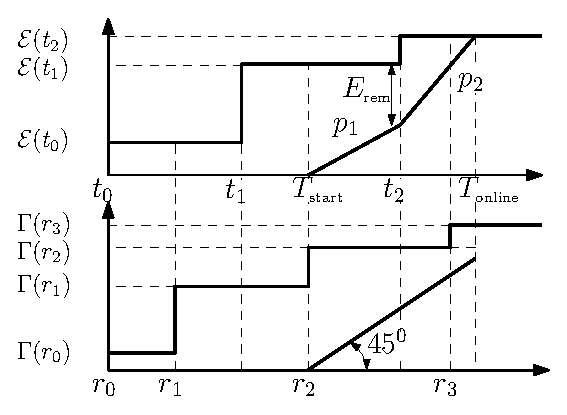
\includegraphics[width=8cm]{online.eps}}
\caption{Example showing execution of the online algorithm. $E_{\mbox{\scriptsize{rem}}}$ value is marked at time $t_2$.}\label{figure_online_example}
\end{figure}


%\begin{algorithm}
%\caption {On-line Algorithm for energy harvesting transmitter and receiver.}
%\footnotesize
%\label{algo_online}
%\begin{algorithmic}[1]
%\State \textbf{Input}: Bits to transmit $B_0$; $\ETx_i$, $\TRx_i$ for $t_i,r_i<t$ where $t$ is the present time instant which increments parallely with this algorithm. 
%
%\State $T_{\mbox{\scriptsize{start}}}=\min\ t$ s.t. $\TRx(t)g\Bigg{(} \dfrac{\ETx(t)}{\TRx(t)}\Bigg{)}\ge B_0$
%\State $B_{\mbox{\scriptsize{rem}}}=B_0$, $E_{\mbox{\scriptsize{rem}}}=\ETx(T_{\mbox{\scriptsize{start}}})$, $m=T_{\mbox{\scriptsize{start}}}$
%
%\Do
%	\State Transmit at power $p$ such that $\dfrac{E_{\mbox{\scriptsize{rem}}}}{p} g(p)= B_{\mbox{\scriptsize{rem}}}$
%	\If {$t=t_i$ for some $i$} 
%		\State $B_{\mbox{\scriptsize{rem}}}=B_{\mbox{\scriptsize{rem}}}-(t_i-m)g(p)$
%		\State $E_{\mbox{\scriptsize{rem}}}=E_{\mbox{\scriptsize{rem}}}+\ETx_i-(t_i-m)p$
%		\State $m=t_i$
%	\EndIf
%\DoWhile {$t\le \left( m+\dfrac{E_{\mbox{\scriptsize{rem}}}}{p}\right)$}
%\end{algorithmic}
%\end{algorithm}

\begin{lemma}
The transmission power in the on-line algorithm is non-decreasing with time.
\label{online_power}
\end{lemma}
%\begin{proof}
%From the definition of the algorithm, the transmission power only changes at energy arrival in transmitter, after $T_{\mbox{\scriptsize{start}}}$. 
%
%Suppose there are energy arrivals after $T_{\mbox{\scriptsize{start}}}$ and for any energy arrival (say $E_{\mbox{\scriptsize{new}}}$) the power changes from $p_i$ to $p_{i+1}$. Let the energy remaining at start of transmission with power $p_i$ be $E_{\mbox{\scriptsize{rem}}}$ and bits remaining be $B_{\mbox{\scriptsize{rem}}}$. The transmission continues for time $l_i$ with power $p_i$. Now, we need to show that $p_i<p_{i+1}$. From the algorithm we get the following equations.  
%\begin{align}
%&\frac{g(p_i)}{p_i}=\frac{B_{\mbox{\scriptsize{rem}}}}{E_{\mbox{\scriptsize{rem}}}} \label{power_increasing_eq1},
%\\
%&\frac{g(p_{i+1})}{p_{i+1}}=\frac{B_{\mbox{\scriptsize{rem}}}-g(p_i) l_i}{E_{\mbox{\scriptsize{rem}}}+E_{\mbox{\scriptsize{new}}}-p_i l_i}.\label{power_increasing_eq2}
%\end{align}
%
%Substituting $g(p_i)$ from (\ref{power_increasing_eq1}) into RHS of (\ref{power_increasing_eq2}), we can see that $\frac{g(p_i)}{p_i}>\frac{g(p_{i+1})}{p_{i+1}}$. Hence, by monotonicity of $g(p)/p$ from \eqref{property_decreasing}, we know that $p_i<p_{i+1}$.
%\end{proof}

\begin{lemma}
In the online policy, if the transmission power at time $t$ is $p$, then $\dfrac{\ETx(t)}{{p}}g(p) \le B_0\;\;\forall\;\; t\in [T_{\mbox{\scriptsize{start}}}, T_{\mbox{\scriptsize{online}}}]$ with equality at $t=T_{\mbox{\scriptsize{start}}}$.
\label{lemma_online_inequality}
\end{lemma}


%\begin{lemma}
%In the online policy $\{\bm{p},\bm{s},N\}$, $\dfrac{g(p_i)}{p_i}\le \dfrac{B_0}{\ETx(s_i)}$.
%\label{lemma_online_inequality}
%\end{lemma}


\begin{proof}
Suppose the online policy is denoted by $\{\bm{p},\bm{s},N\}$. It is then enough to prove that $\frac{g(p_i)}{p_i} \le \frac{B_0}{\ETx(s_i)}$ for $i\in\{1,..,N\} $, because both $p_i$ and $\ETx(t)$ remains constant in $t\in[s_i,s_{i+1})$. We prove it by induction on $i$ in ordered set $\{1,2..,N\}$. 

With $s_1=T_{\mbox{\scriptsize{start}}}$, the base case follows form equality \eqref{eq_online_first_power}. Now, assume $\frac{g(p_i)}{p_i}\le \frac{B_0}{\ETx(s_i)}$ to be true for $i=k-1$, $k\in \{2,..,N\}$. Let $E_{\mbox{\scriptsize{rem}}}$ and $B_{\mbox{\scriptsize{rem}}}$ be the residual energy and bits, at time $s_{k-1}$. As $s_k=t_j$ for some $j$, we can write,
\begin{align*}
&\frac{p_{k}}{g(p_{k})}=\frac{E_{\mbox{\scriptsize{rem}}}+E_{j}-p_{k-1} (s_k-s_{k-1})}{B_{\mbox{\scriptsize{rem}}}-g(p_{k-1}) (s_k-s_{k-1})},
\\
&\stackrel{(a)}{=}\frac{p_{k-1}}{g(p_{k-1})}+\frac{E_{j}}{B_{\mbox{\scriptsize{rem}}}\gamma}
\stackrel{(b)}{>}\frac{\ETx(s_{k-1})}{B_0}+\frac{E_{j}}{B_0}=\frac{{\ETx(s_{k})}}{B_0}.
\end{align*}

where $(a)$ follows form $\frac{B_{\mbox{\scriptsize{rem}}}}{E_{\mbox{\scriptsize{rem}}}}=\frac{g(p_{k-1})}{p_{k-1}}$ and substitution $\gamma=\left( 1-\frac{p_{k-1}}{E_{\mbox{\scriptsize{rem}}}} (s_k-s_{k-1})\right)< 1$;  $(b)$ uses induction hypothesis along with the inequality $B_{\mbox{\scriptsize{rem}}}\gamma< B_0$. This completes the proof of Lemma \ref{lemma_online_inequality}. From equality $(a)$ we can see that $g(p_k)/p_k<g(p_{k-1})/p_{k-1}$. Hence, by monotonicity of $g(p)/p$, $p_{k}>p_{k-1}$. This proofs Lemma \ref{online_power}.
\end{proof}



\begin{lemma}
The online policy starts atleast by the time the optimal offline policy ends i.e. $T_{\mbox{\scriptsize{start}}} <T_{\mbox{\scriptsize{off}}}$.
\label{onilne_time}
\end{lemma}


\begin{proof}
We will prove this by contradiction. Suppose $T_{\mbox{\scriptsize{start}}} \ge T_{\mbox{\scriptsize{off}}}$. From \eqref{online_T_start}, either $T_{\mbox{\scriptsize{start}}}=t_i$ for some $i$ and/or $T_{\mbox{\scriptsize{start}}}=r_j$ for some $j$.

If $T_{\mbox{\scriptsize{start}}}=t_i$, then %as $T_{\mbox{\scriptsize{off}}}\le T_{\mbox{\scriptsize{start}}}$, 
the maximum energy that can be utilized by the offline policy is $\ETx(T_{\mbox{\scriptsize{start}}}^-)=\TRx(T_{\mbox{\scriptsize{start}}})-\ETx_i\neq \TRx(T_{\mbox{\scriptsize{start}}})$.
%Note that the offline policy cannot use energy arrival $\ETx_i$, as using any finite amount of energy for 0 time cannot deliver any bits. 

If $T_{\mbox{\scriptsize{start}}}=r_j$, then the maximum time for which the receiver can be \textit{on} in the offline policy is $\TRx(T_{\mbox{\scriptsize{start}}}^-)=\TRx(T_{\mbox{\scriptsize{start}}})-\TRx_j\neq \TRx(T_{\mbox{\scriptsize{start}}})$.
%, as the offline policy has to finish at or before $T_{\mbox{\scriptsize{start}}}$. 
%Note that, in the optimal offline policy, time for which the receiver is \textit{on} is given by $\displaystyle \sum_{i:p_i\neq 0}(s_{i+1}-s_i)$. 

%If $T_{\mbox{\scriptsize{start}}}\neq t_i$ or $T_{\mbox{\scriptsize{start}}}\neq r_j$ then, $\ETx(T_{\mbox{\scriptsize{start}}}^-)=\ETx(T_{\mbox{\scriptsize{start}}})$ or $\TRx(T_{\mbox{\scriptsize{start}}}^-)=\TRx(T_{\mbox{\scriptsize{start}}})$.

Now, the number of bits transmitted by the offline policy $\{\bm{p},\bm{s},N\}$ is given by,
\begin{align}
&\sum_{{\substack{i=1\\p_i\neq 0}}}^{i=N} g(p_i)(s_{i+1}-s_{i}),
\\
&\nonumber \stackrel{(a)}{\le}g\left(\frac{\displaystyle\sum_{i:p_i\neq 0}p_i(s_{i+1}-s_{i})}{\displaystyle\sum_{j:p_j\neq 0}(s_{j+1}-s_{j})}\right)\sum_{j:p_j\neq 0} (s_{j+1}-s_{j}),
\\
&\stackrel{(b)}\le g\left(\frac{\ETx(T_{\mbox{\scriptsize{start}}}^-)}{\TRx(T_{\mbox{\scriptsize{start}}}^-)}\right)\TRx(T_{\mbox{\scriptsize{start}}}^-)\stackrel{(c)}{<}B_0.\label{online_eq_2}
\end{align}
%%%&\nonumber\stackrel{(b)}{\le} g\left( \frac{\displaystyle\sum_{i:p_i\neq 0} p_i(s_{i+1}-s_{i})}{\TRx(T_{\mbox{\scriptsize{start}}}^-)} \right)\TRx(T_{\mbox{\scriptsize{start}}}^-), 
%%%&\nonumber\stackrel{(a)}{\le} g\left(\sum_{\substack{i\\p_i\neq 0}}p_i\left(\frac{(s_{i+1}-s_{i})}{\displaystyle\sum_{j:p_j\neq 0}(s_{j+1}-s_{j})}\right)\right) \sum_{\substack{j\\p_j\neq 0}} (s_{j+1}-s_{j}),

where $(a)$ follows from application of Jensen's inequality due to concavity of $g(p)$; $(b)$ follows form the fact that $\displaystyle\sum_{j:p_j\neq 0}(s_{j+1}-s_{j})\le\TRx(T_{\mbox{\scriptsize{off}}})\le \TRx(T_{\mbox{\scriptsize{start}}}^-)$ and $g(p)/p$ is monotonically decreasing; $(c)$ follows form \eqref{online_T_start}. \eqref{online_eq_2} implies that the number of bits transmitted by the offline policy is less than $B_0$. Therefore, by contradiction, $T_{\mbox{\scriptsize{start}}}<T_{\mbox{\scriptsize{off}}}$.
\end{proof}



\begin{theorem}
The competitive ratio of the online policy is strictly less than 2.
\end{theorem}
\begin{proof}
%This is equivalent to saying that the time taken by the online policy can at max be approaching twice the time taken by optimal offline policy, over all possible energy arrival sequences. Let the time taken by the optimal offline policy be $T_{\mbox{\scriptsize{off}}}$ and the online policy, say $\{\bm{{p}},\bm{{s}},{N}\}$, be $T_{\mbox{\scriptsize{online}}}$. Note that $s_{N+1}=T_{\mbox{\scriptsize{online}}}$. 

The idea behind the proof is to show that the online policy can conitnue for at max $T_{\mbox{\scriptsize{off}}}$ time  after the offline policy ends.

Let the online policy be $\{\bm{{p}},\bm{{s}},{N}\}$ ($s_1=T_{\mbox{\scriptsize{start}}}, s_{N+1}=T_{\mbox{\scriptsize{online}}}$). Consider the transmission power of the online policy just before $T_{\mbox{\scriptsize{off}}}$. This will be non zero as $T_{\mbox{\scriptsize{start}}}<T_{\mbox{\scriptsize{off}}}$ from Lemma \ref{onilne_time}. Let it be ${p}_l$. So, $s_l<T_{\mbox{\scriptsize{off}}}$. Let $E_{\mbox{\scriptsize{rem}}}$ and $B_{\mbox{\scriptsize{rem}}}$ denote the residual energy and bits at time ${s}_{l}$.
% Note that, either ${s}_{l}=T_{\mbox{\scriptsize{start}}}$ or ${s}_{l}=t_k$ for some $k$. 
%Also, 
%\begin{align}
%&\ETx({s}_{l})=\ETx(T_{\mbox{\scriptsize{off}}}^-),
%\label{eq_online_time_0}
%\end{align}
%because if $s_{l}=t_k$, $t_k$ would be the last energy arrival epoch before $T_{\mbox{\scriptsize{off}}}$ or $s_l=T_{\mbox{\scriptsize{start}}}$, then $T_{\mbox{\scriptsize{start}}}$ would be greater than or equal to the last energy arrival epoch before $T_{\mbox{\scriptsize{off}}}$. 

Since the number of bits sent by online policy after ${s}_l$ is equal to $B_{\mbox{\scriptsize{rem}}}$, by Lemma \ref{online_power},
\begin{align}
&\sum_{i=l}^{i={N}}g(p_i)({s}_{i+1}-{s}_i)=B_{\mbox{\scriptsize{rem}}},
\\
&({s}_{{N}+1}-{s}_l)\le\frac{B_{\mbox{\scriptsize{rem}}}}{g(p_l)}=\frac{E_{\mbox{\scriptsize{rem}}}}{p_l}\le \frac{\ETx({s}_l)}{p_l}\le \frac{\ETx(T_{\mbox{\scriptsize{off}}}^-)}{p_l}.
\label{eq_online_time_1}  
\end{align}
Applying Lemma \ref{lemma_online_inequality} at time $T_{\mbox{\scriptsize{off}}}^-$,
\begin{align}
&\frac{\ETx(T_{\mbox{\scriptsize{off}}}^-)}{p_l}g(p_l)\le B_0\stackrel{(a)}{\le}T_{\mbox{\scriptsize{off}}}\; g\left(\frac{\ETx(T_{\mbox{\scriptsize{off}}}^-)}{T_{\mbox{\scriptsize{off}}}}\right),
\label{eq_online_time_2}
\end{align}
where $(a)$ holds because the maximum bits sent by the offline policy can be bounded by $T_{\mbox{\scriptsize{off}}}\; g\left(\frac{\ETx(T_{\mbox{\scriptsize{off}}}^-)}{T_{\mbox{\scriptsize{off}}}}\right)$ due to concavity of $g(p)$. By monotonicity property of $g(p)/p$ in \eqref{property_decreasing}, we can conclude from \eqref{eq_online_time_2} that, $\frac{\ETx(T_{\mbox{\scriptsize{off}}}^-)}{p_l}\le T_{\mbox{\scriptsize{off}}}$. 
%Hence, using \eqref{eq_online_time_0}, we get, $\frac{\ETx({s}_l)}{p_l}\le T_{\mbox{\scriptsize{off}}}$. 
Combining this with \eqref{eq_online_time_1},
\begin{align}
&({s}_{{N}+1}-{s}_l)\le T_{\mbox{\scriptsize{off}}}.
\label{eq_online_time_3}
\end{align} 

Finally, we can calculate the competitive ratio as,
\begin{align*}
&r=\displaystyle\max_{\ETx(t),\TRx(t)\hspace{0.5mm} \forall t}\dfrac{T_{\mbox{\scriptsize{online}}}}{T_{\mbox{\scriptsize{off}}}} = \dfrac{({s}_{{N}+1}-{s}_l)+{s}_l}{T_{\mbox{\scriptsize{off}}}} \stackrel{(a)}{<} 2,
\end{align*}
where $(a)$ follows from \eqref{eq_online_time_3}, and ${s}_l<T_{\mbox{\scriptsize{off}}}$.        
\end{proof}
\appendices
\bibliographystyle{IEEEtran}
\bibliography{refs_TIFR_intern}
 
\end{document}
